\section{Tools to support the project management}
\label{ProjMgmtTools}
This section lists the tools used during the project for reasons of transparency. It also allows the reader to evaluate different ways in which these tools can be used. 

\subsection*{Miro}
\label{ProjMgmtToolMiro}
Miro is part of the toolset of both the academic team and the Swiss Post teams. However, in this project, it was used only by the academic team. The reason for using Miro is that it is a lightweight tool that allows combining different data structures on a single board. Miro provides an infinite canvas on which a wide variety of information can be placed. The information can be structured and easily rearranged to regroup related elements. This allows the tool to be used both for early documentation of information and for later restructuring when additional ideas emerge, particularly in the context of long-term documentation. The ability to restructure information visually supports the decomposition and understanding of complex environments.

A full set of screenshots illustrating changes on the Miro board has been moved to the Annex, while the final one is included here (Appendix \ref{apendixMiroUsage}). The following screenshot represents the Miro board during the finalisation of the document, zoomed out so that all elements are visible. While this view prevents individual details from being seen, some relevant parts are shown in detail in the following subsubsections.

\begin{figure}[H]
    \centering
    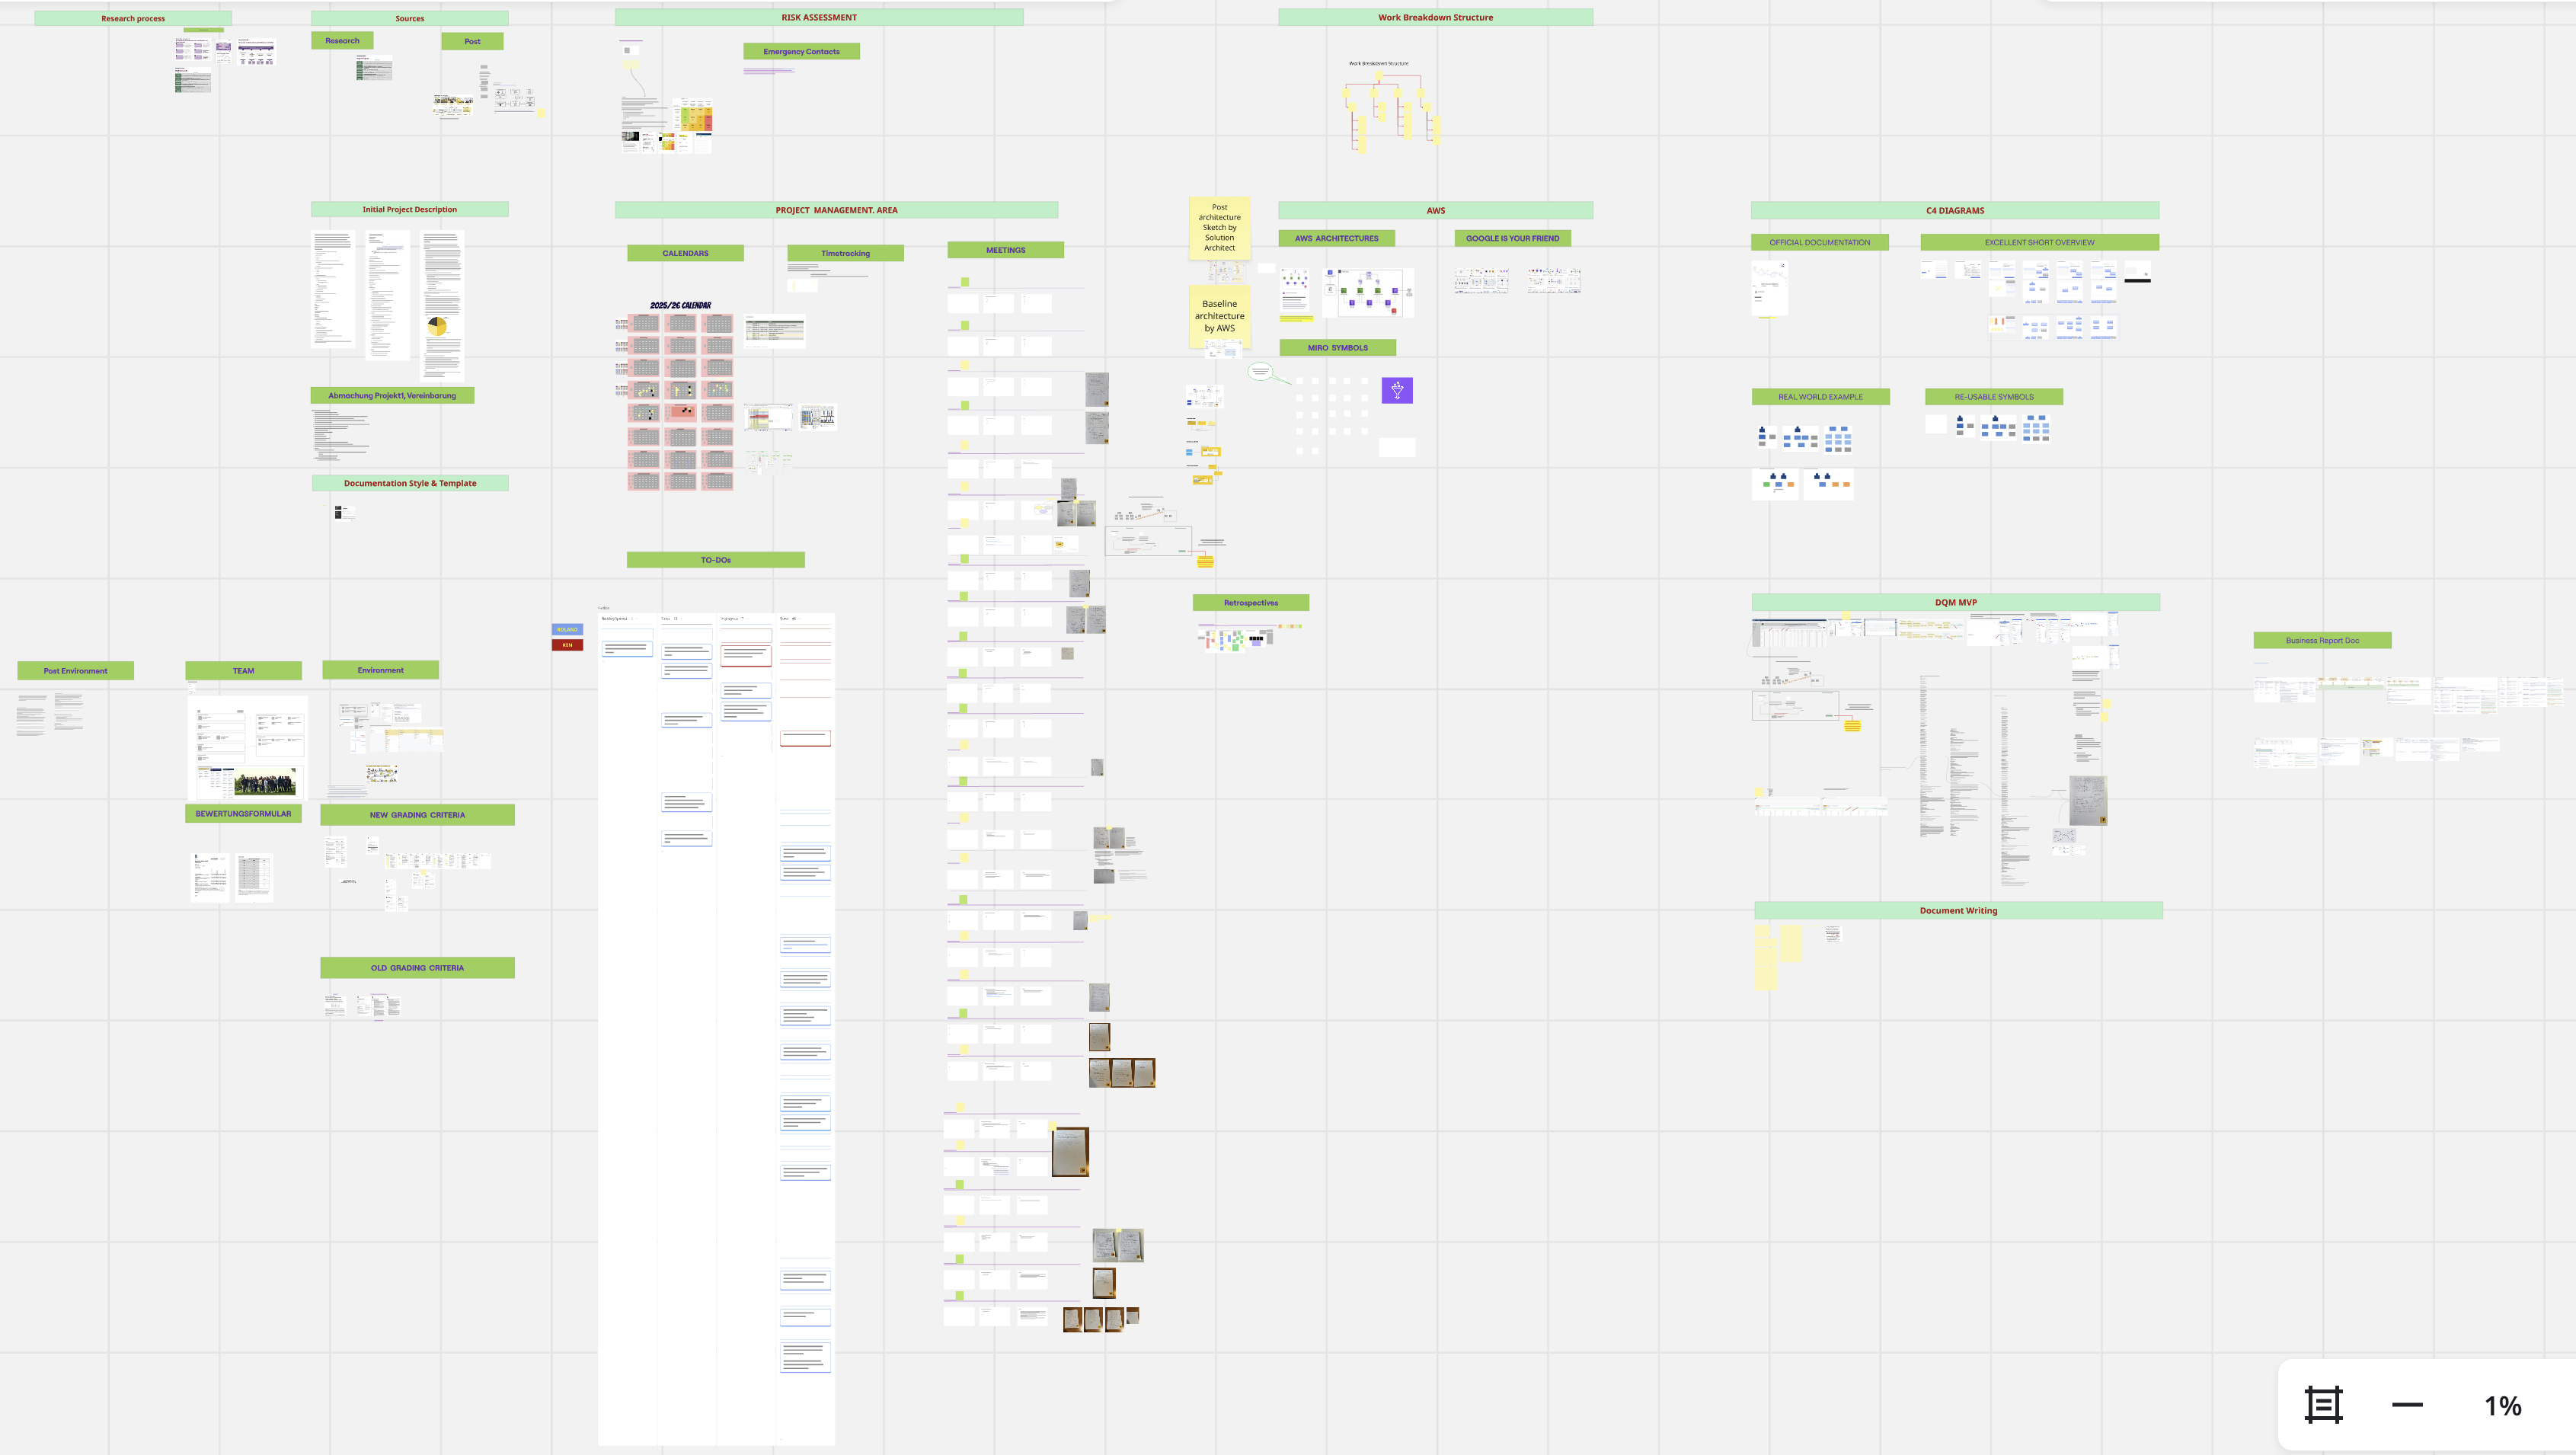
\includegraphics[width=0.8\textwidth]{./content/img/MiroBoard_23-12-2025.png}
    \caption{Miro board documentation, view of 23.12.2025}
    \label{fig:miro_final_board_twentythird_december}
\end{figure}

\subsubsection*{Miro calendar}
The calendar in Miro was primarily used to schedule the milestones. These are shown with green tiles on the corresponding dates, including their number and milestone title. Jour Fixe meetings are marked in yellow whenever they occurred, including adjustments in cases of unavailability. Actual unavailabilities at scheduled Jour Fixe meetings and other times are documented in black. Finally, holidays are marked in teal. In the case of this project, this applied only to the Christmas and New Year holiday period.

\begin{figure}[H]
    \centering
    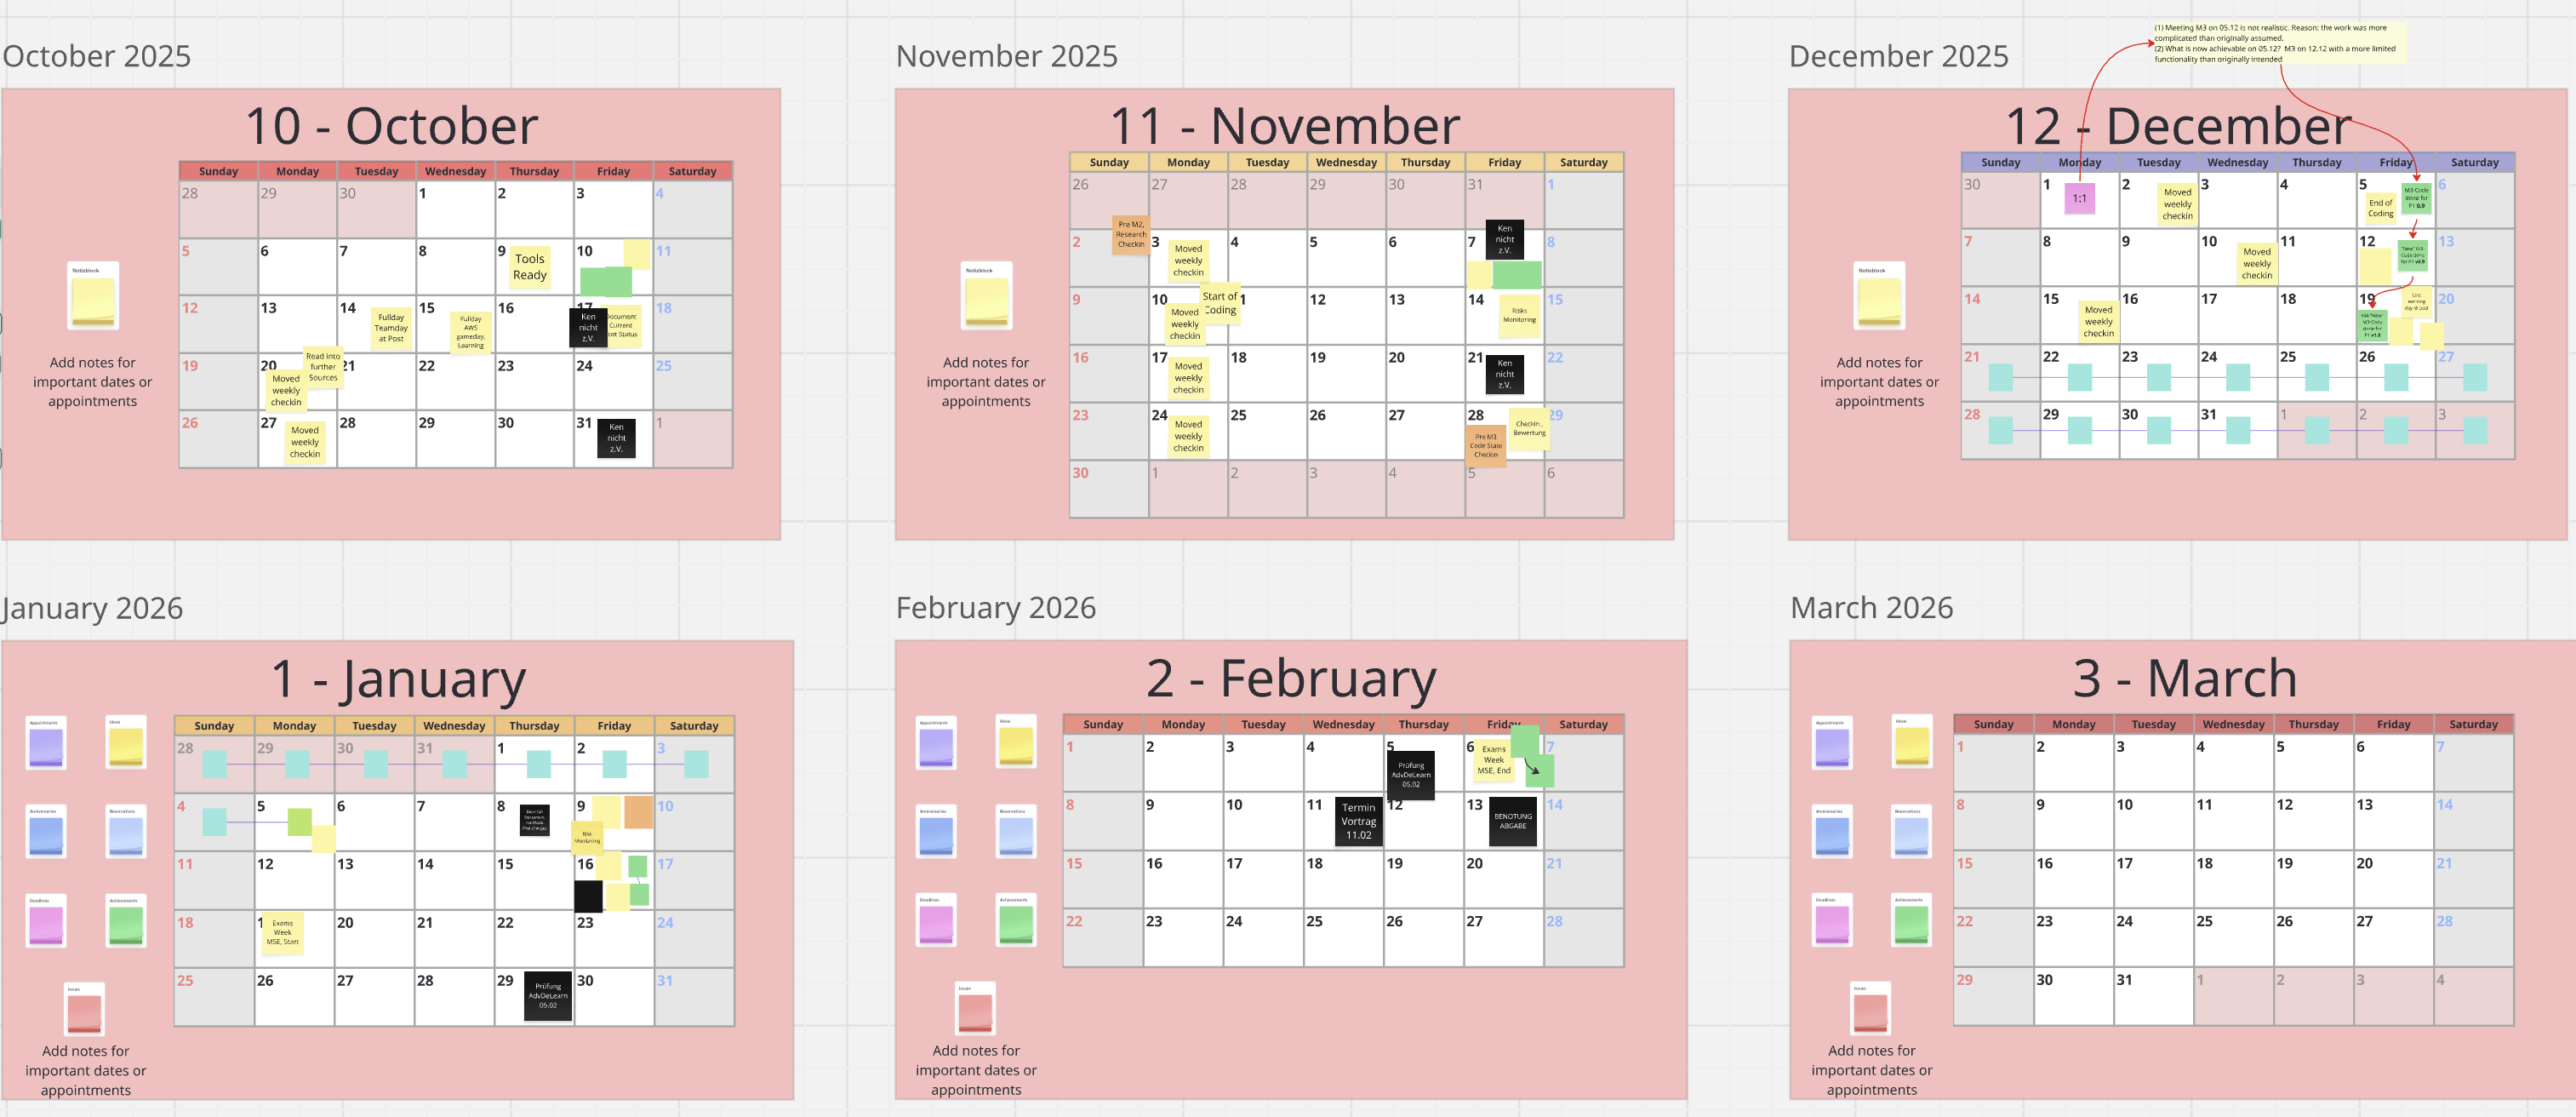
\includegraphics[width=0.8\textwidth]{./content/img/MiroBoard_Calendar.png}
    \caption{Miro board calendar used for coordination and tracking of milestones and related events}
    \label{fig:miro_board_calendar}
\end{figure}

\subsubsection*{Meetings documentation}
The meetings are documented using a layout with three sections, including a coloured tag at the top in yellow for Swiss Post meetings and green for academic ones. From left to right, these sections are structured as follows. First, the meeting points to be discussed are listed; these are copied from the Outlook invitations. Second, the topics addressed are summarised, mostly after the meeting. Third, the to-do block describes any actions that arose during the meeting. Not every meeting includes all sections. Furthermore, meetings are often documented using handwritten minutes. These are uploaded to the right of the meeting blocks without further refinement and serve as references.

\begin{figure}[H]
    \centering
    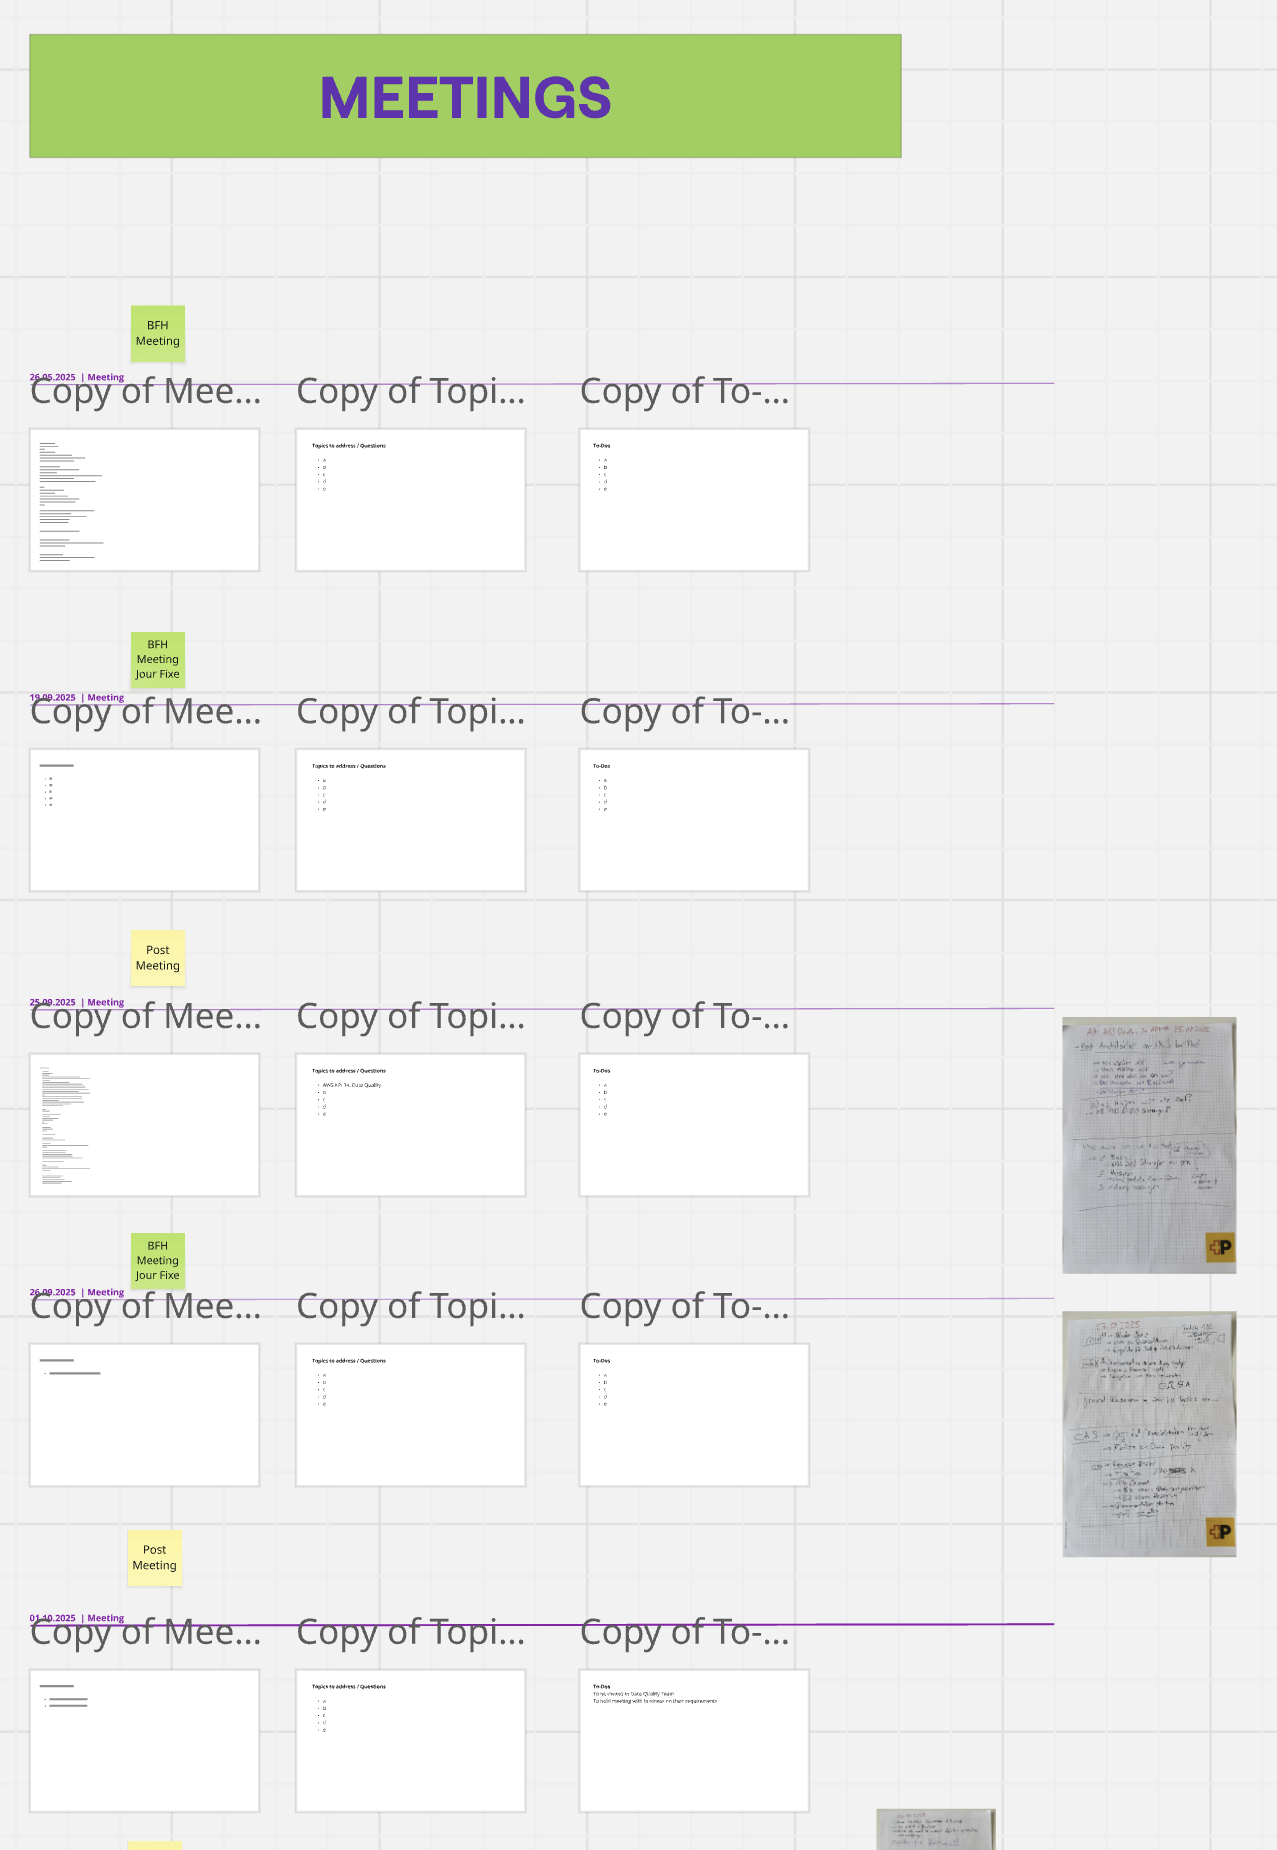
\includegraphics[width=0.8\textwidth]{./content/img/MiroBoard_Meetings.png}
    \caption{Miro board, tracking of meetings: when, who, what}
    \label{fig:miro_board_meetings}
\end{figure}

\subsubsection*{Documentation of the Implementation}
The implementation was first documented in Miro, as the rapid creation of screenshots did not disturb the flow of information gathering. In the following figure, the information-gathering process can be seen, starting from the top left, moving to the right, and then restarting from the left. First, screenshots of the SAC report are shown, followed by navigation towards DSP. Further details on the tools are described in the Implementation chapter.

\begin{figure}[H]
    \centering
    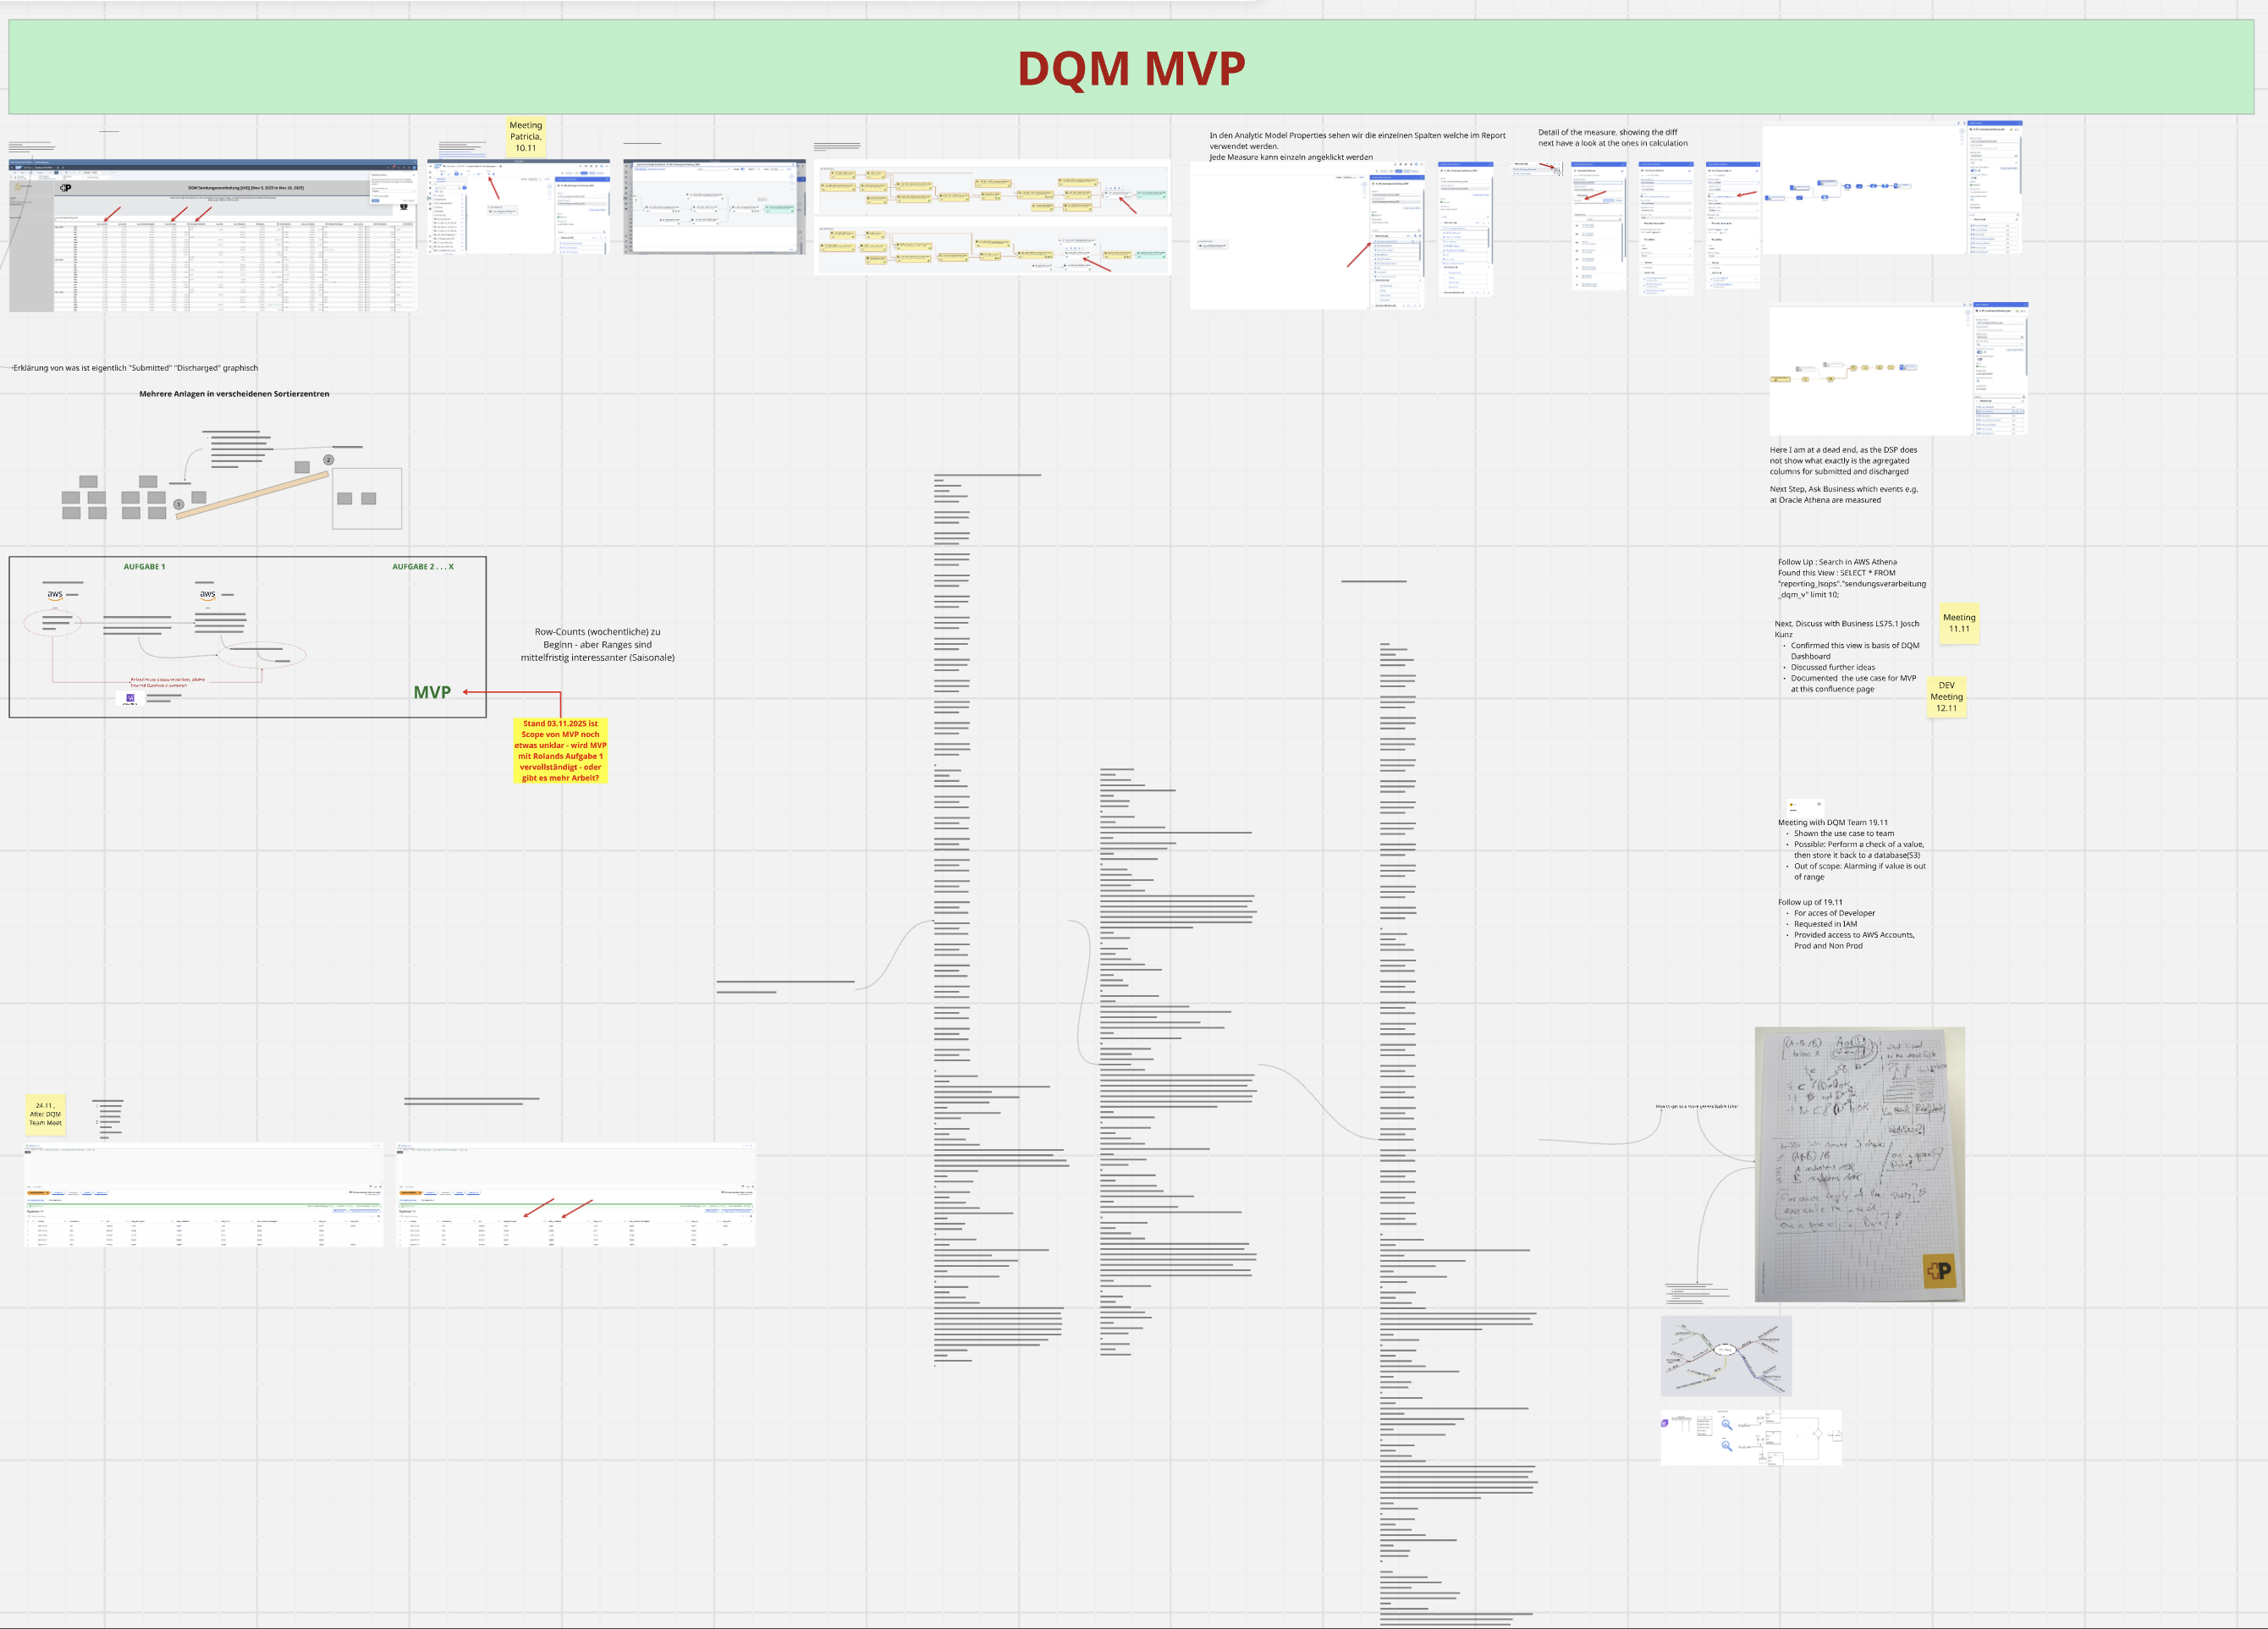
\includegraphics[width=0.8\textwidth]{./content/img/MiroBoard_Implementation.png}
    \caption{Miro board usage for quick documentation during implementation}
    \label{fig:miro_board_implementation}
\end{figure}


\subsection*{Jira and Confluence}

Jira (mainly for issue tracking) and Confluence (mainly for documentation) are both tools provided by Atlassian and are therefore well integrated with each other. The tools are installed on-premises, which limits sharing possibilities outside the Swiss Post network. They are used by the three Swiss Post teams presented in the Teams section. The project team also used Confluence when research results had to be presented as a first use case. While Jira is used for the short-term management of Scrum artefacts, Confluence is used for long-term documentation. An example of such long-term documentation is shown in the following screenshot, illustrating the documentation of a data lineage.

\begin{figure}[H]
    \centering
    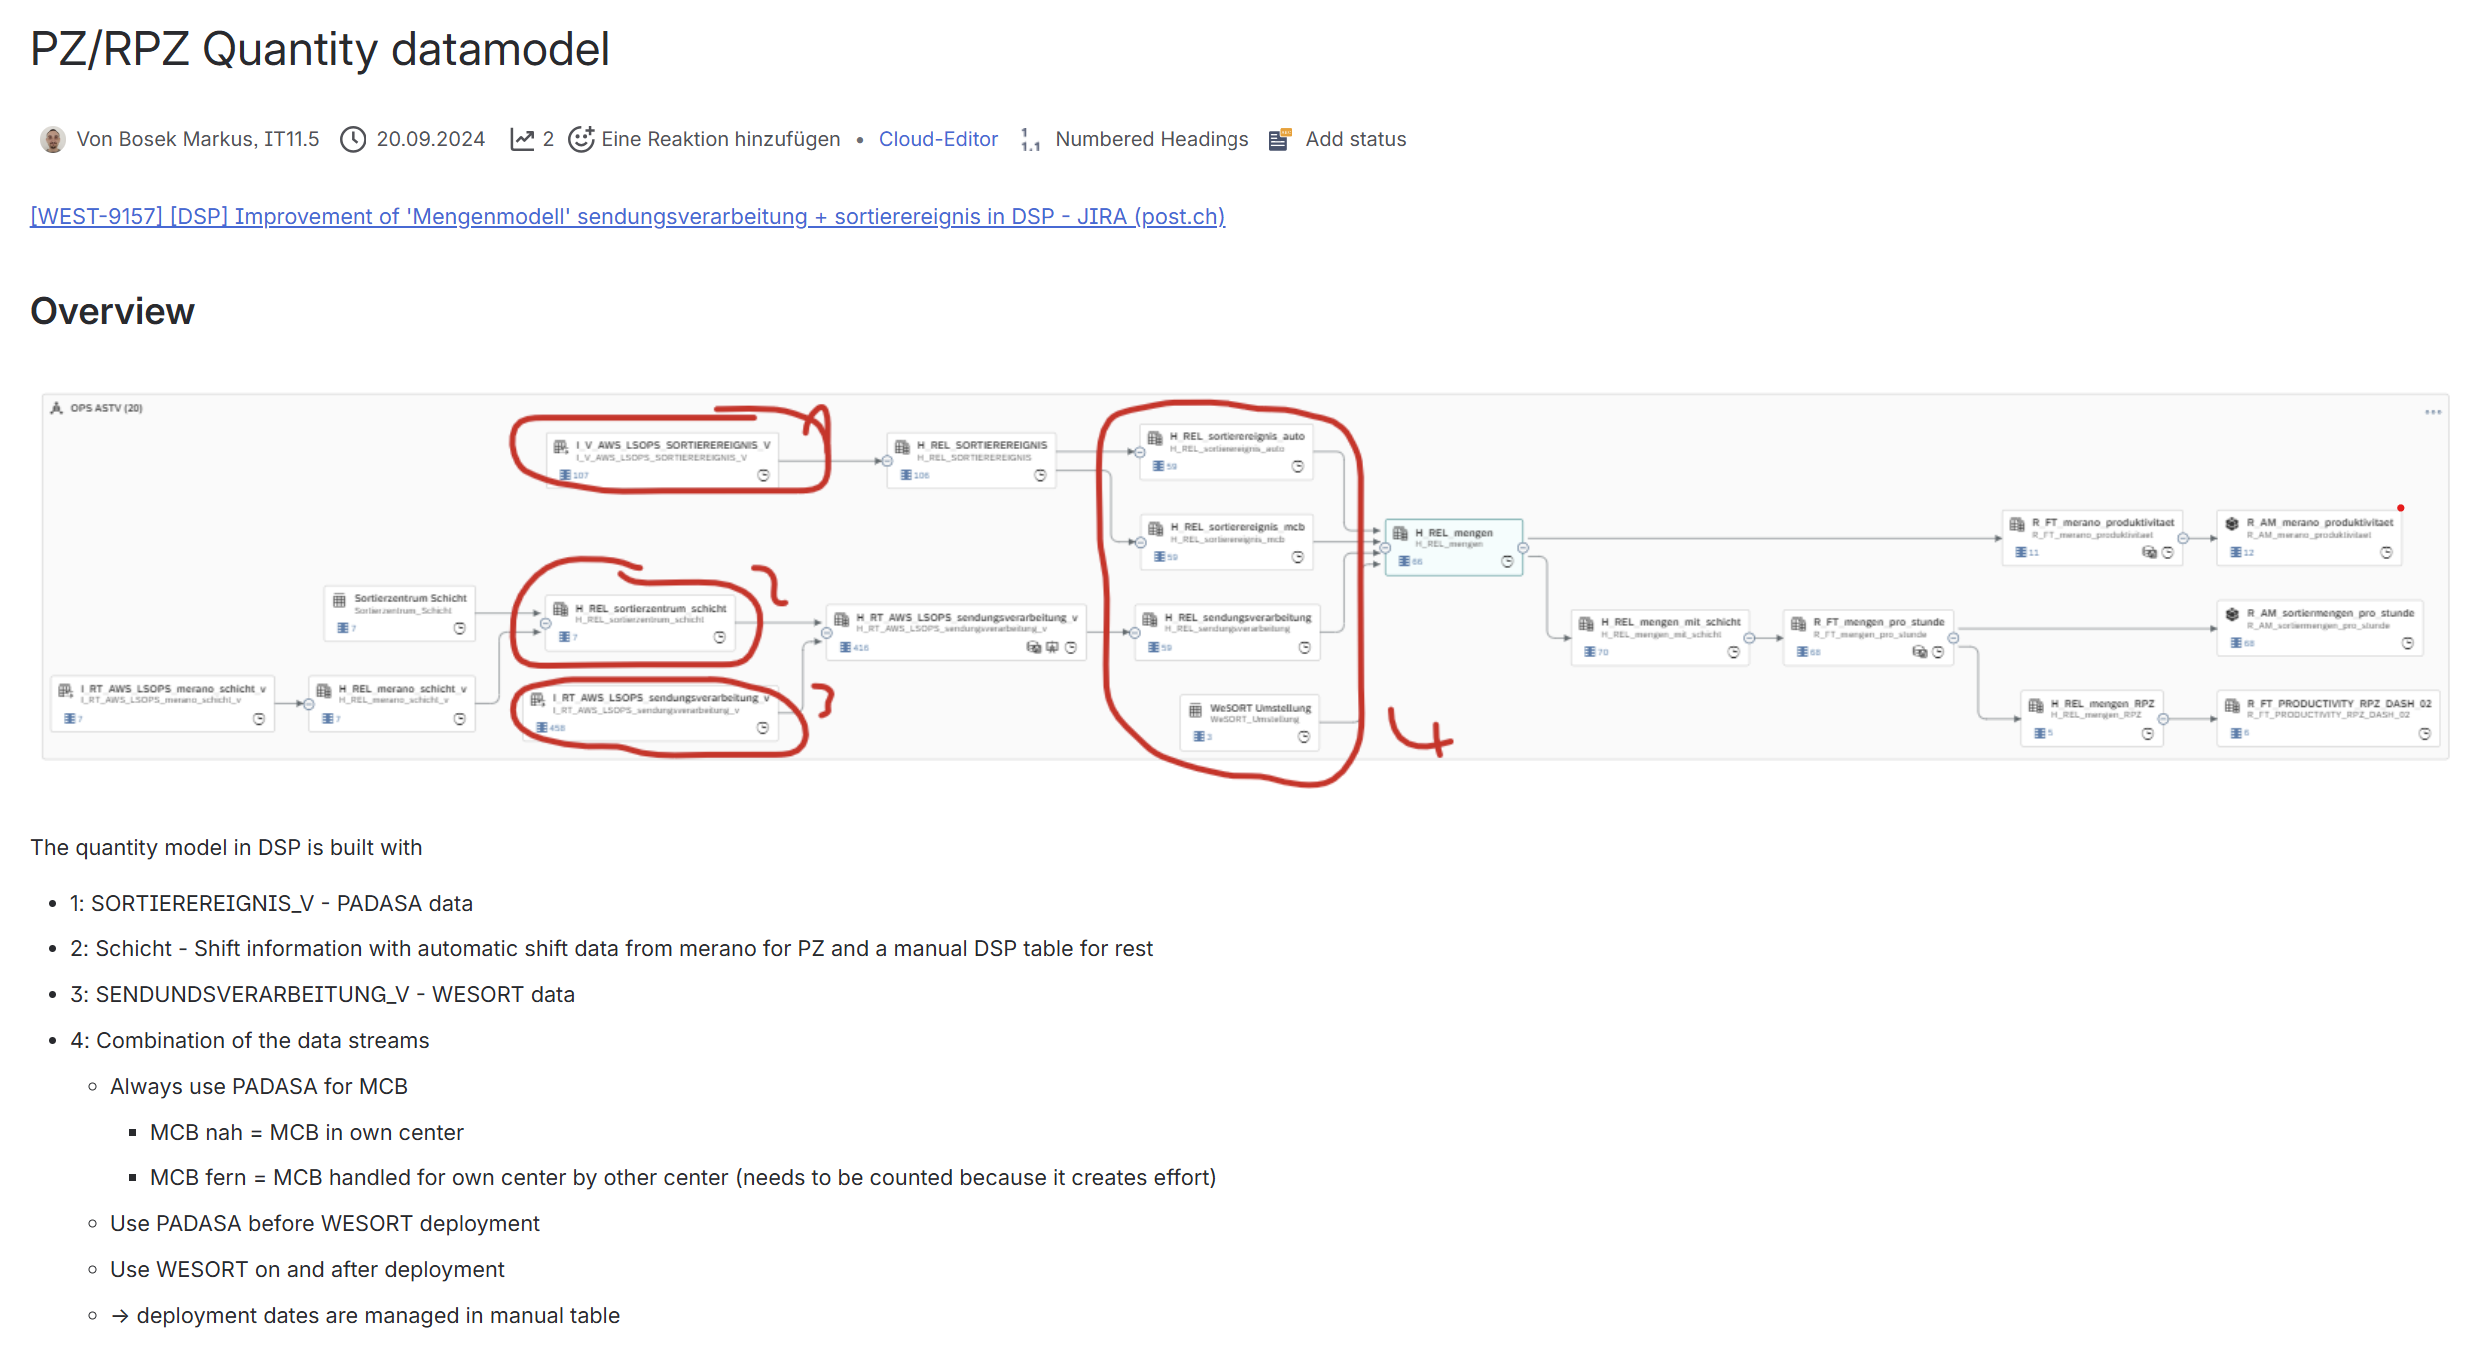
\includegraphics[width=0.95\textwidth]{./content/img/ProjectManagement/Confluence_usage_longtime_documentation.png}
    \caption{Example of project documentation in Confluence used to record architectural decisions and their rationale for future reference}
    \label{fig:confluence_architecture_documentation}
\end{figure}

\subsection*{Microsoft Teams and Microsoft Outlook}
MS Teams and MS Outlook are used by both the academic and Swiss Post teams. They are organisational standards at Swiss Post and are not optional. The same applies to the academic context. Both tools serve to support focused long-term (MS Outlook) and short-term (MS Teams) communication.

\subsection*{Shared chat}
For the academic team, the chat was used for short-term communication. However, a challenge arose due to the involvement of two distinct organisations, BFH and the Swiss Post. In order to keep communication between Swiss Post accounts and BFH accounts in one place, a chat with three users was required. In this context, the cross-organisational capabilities of MS Teams proved useful. After the Swiss Post account was invited to participate in the project team, it was able to communicate directly with BFH accounts. A sample of the communication involving three accounts is shown below.

\begin{figure}[H]
    \centering
    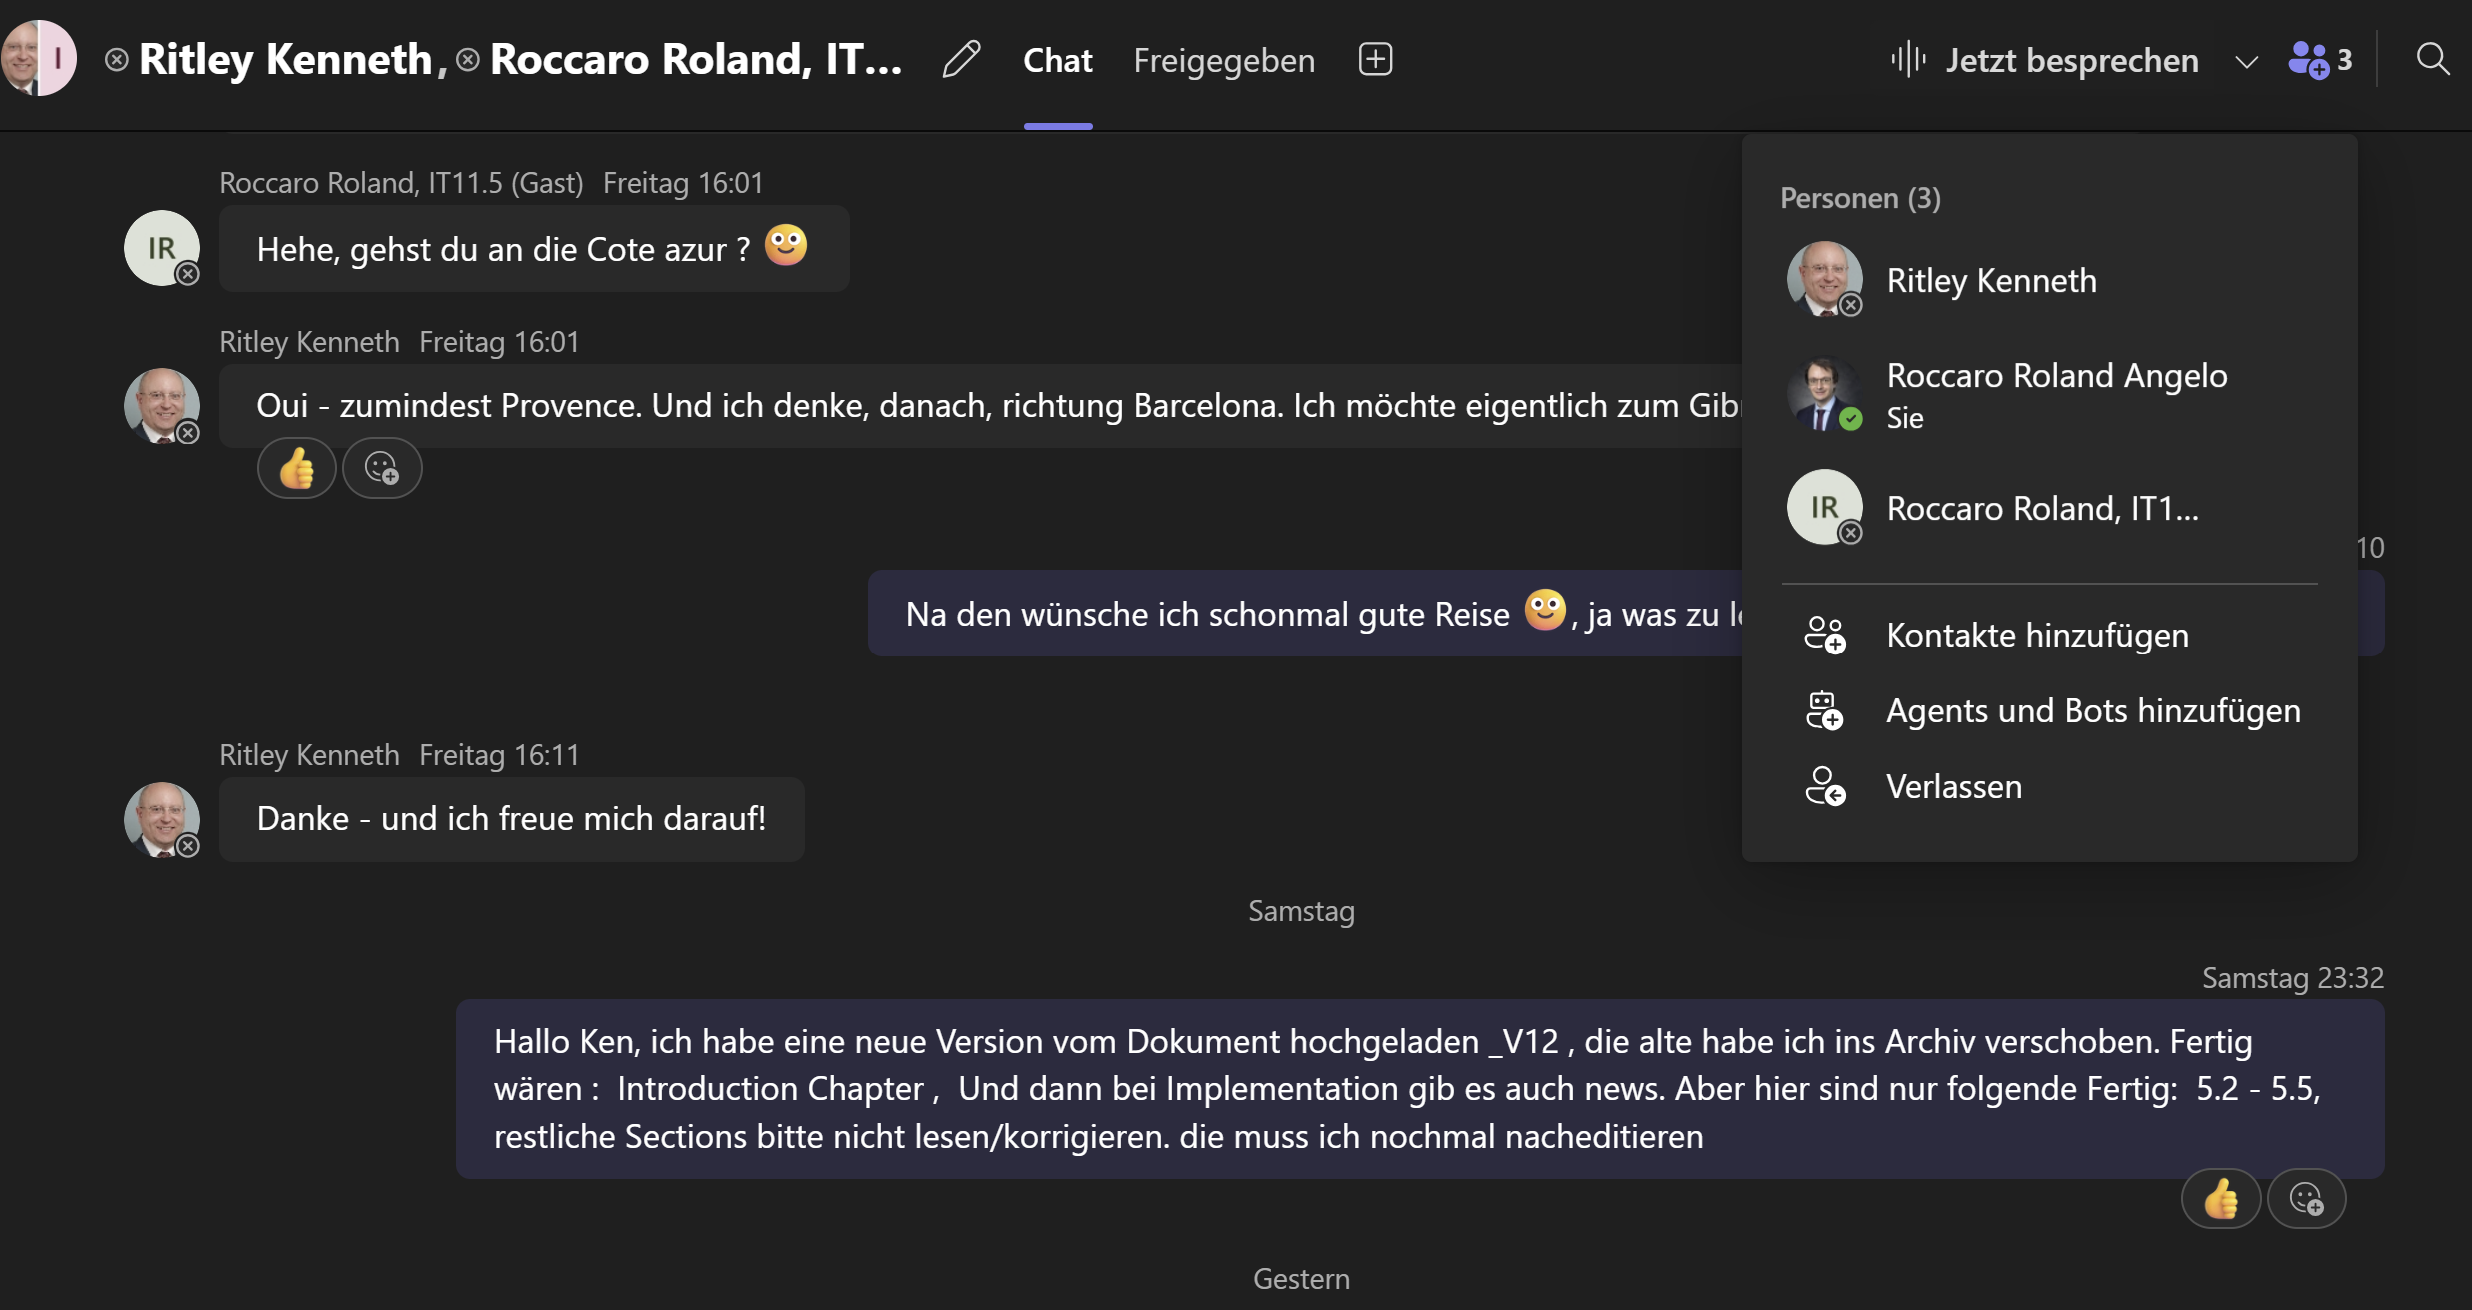
\includegraphics[width=0.8\textwidth]{./content/img/ProjectManagement/ProjMgmt_Teams_Chat.png}
    \caption{Shared chat using Teams}
    \label{fig:teams_shared_chat}
\end{figure}

A second important application of MS Teams is a document management system. This includes source documents, document versions, and related materials. All relevant documents are stored within this structure, which is designed to grow as needed.

\begin{figure}[H]
    \centering
    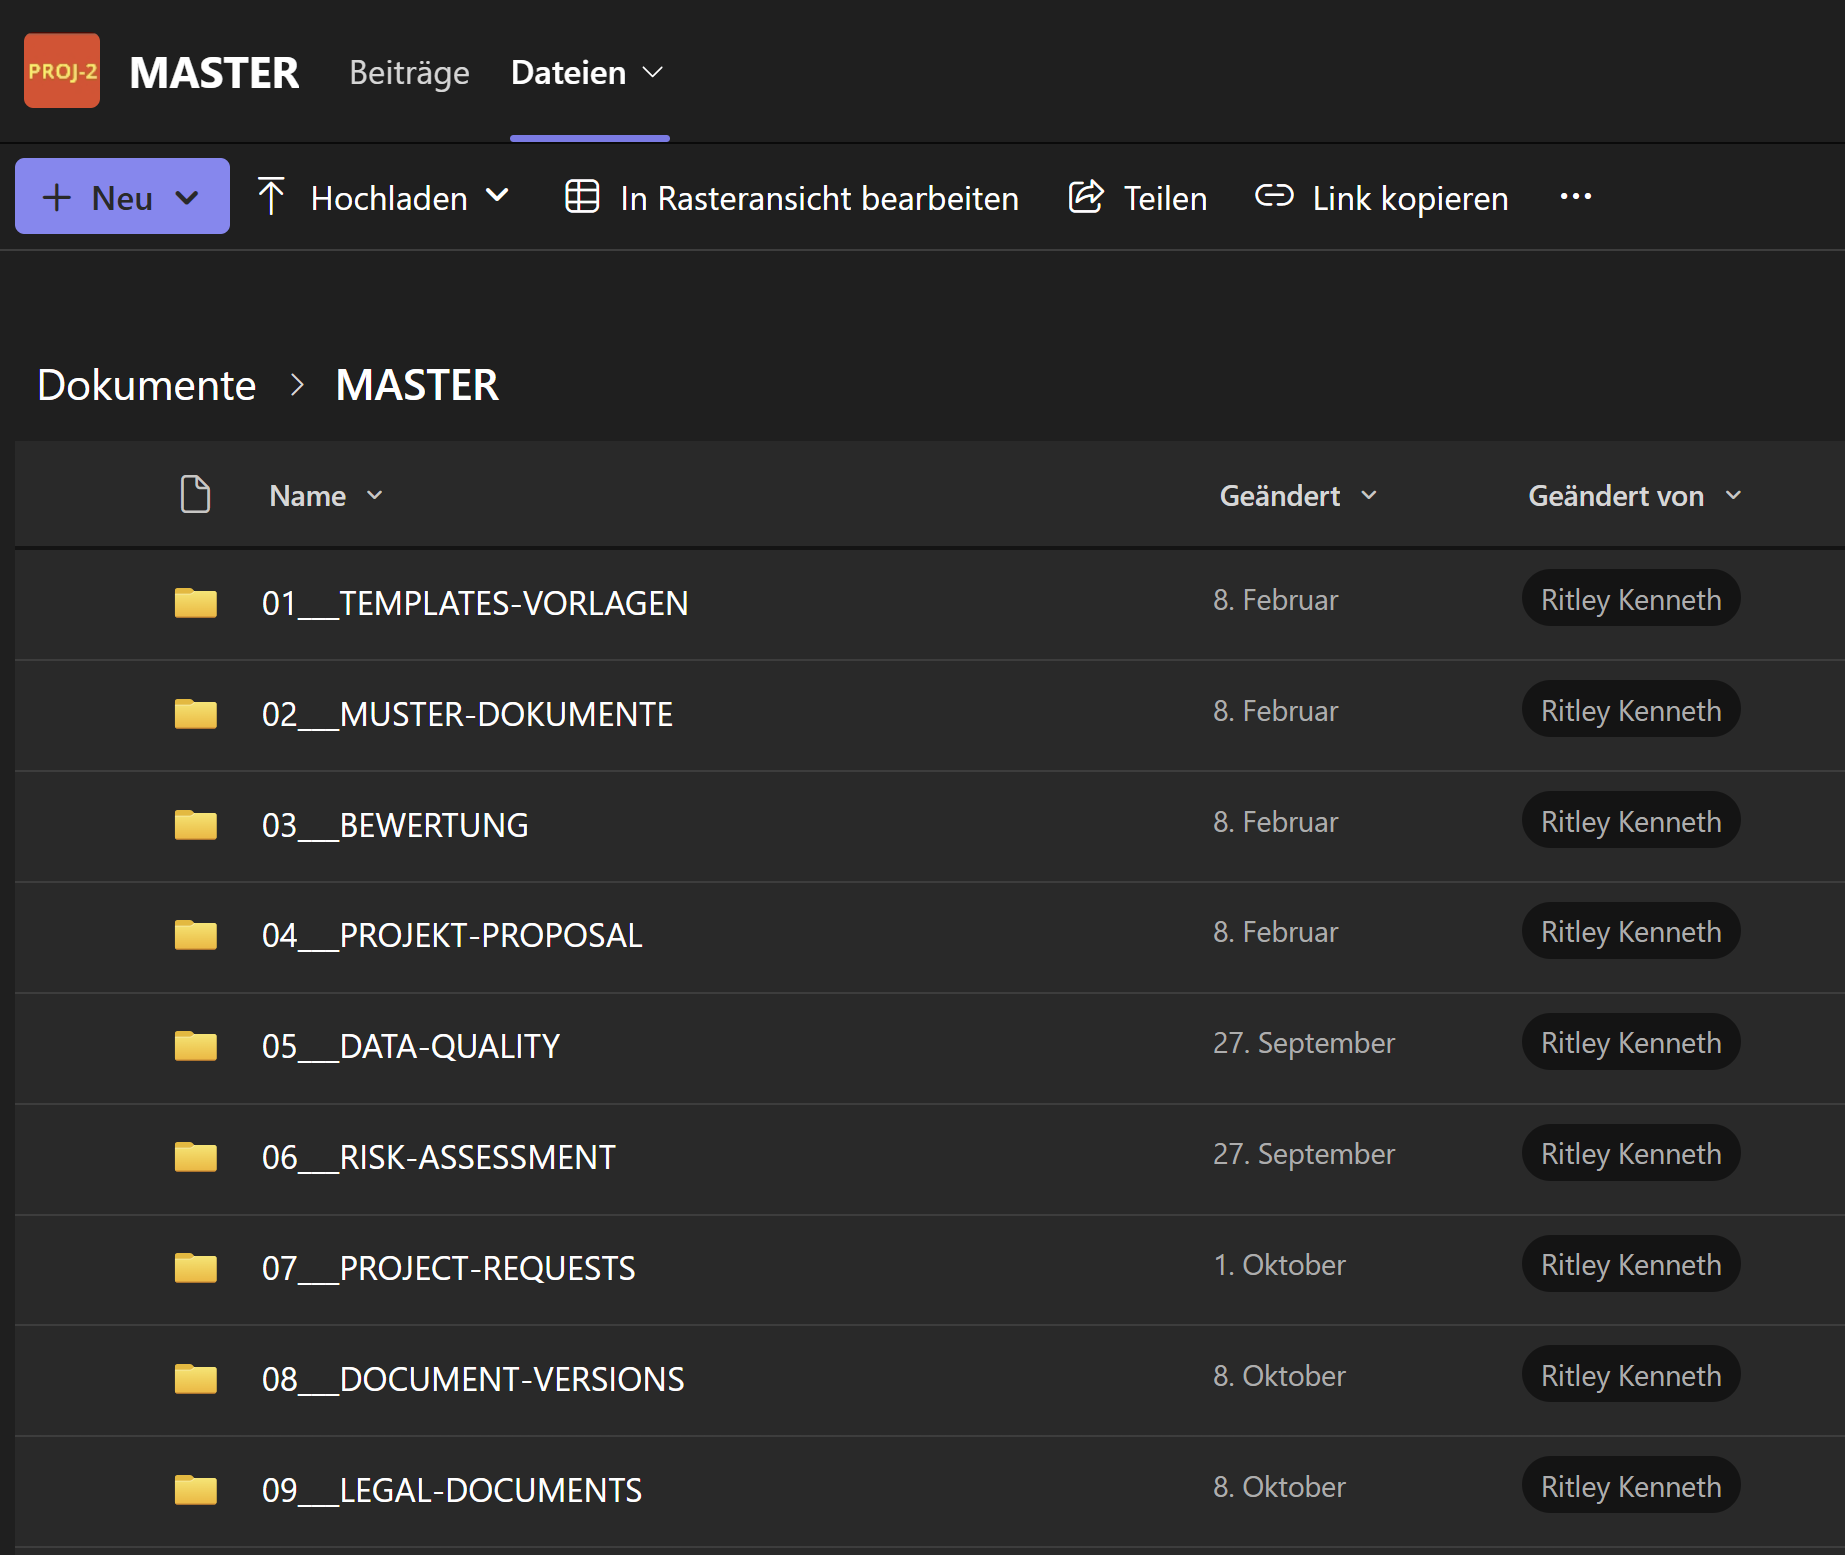
\includegraphics[width=0.8\textwidth]{./content/img/ProjectManagement/ProjMgmt_Teams_Documents.png}
    \caption{Project document store used with Teams}
    \label{fig:teams_document_store}
\end{figure}

\subsection*{LaTeX}
LaTeX was the tool chosen for the main writing process by the academic team. The primary reason for selecting this tool was the consistency of the document structure. It allows changes to be made in a large document without the document becoming unstable. The tool was specifically selected for this higher consistency compared to Word. The fact that the creation of some stylistic elements takes more time than with a \gls{WYSIWYG} editor such as Word was accepted, particularly as design was valued lower than document content. Finally, the consistency of being able to reference text sections within the document and the ability to automatically generate lists of figures and tables were seen as additional benefits. Furthermore, the automatic glossary and citation features using Biber were considered advantages for which the slower writing process without a WYSIWYG editor was accepted. Due to the learning effort involved in using \LaTeX, the following badge was earned during the course of the research.

\begin{figure}[H]
    \centering
    
\includegraphics[width=0.65\textwidth]{./content/img/ProjectManagement/RolandMasterOfLatex.png}
    \caption{Humorous illustration symbolising the extensive use of \LaTeX\ throughout the preparation of this report and the associated learning experience during the project.}
    \label{fig:latex_mastery}
\end{figure}

\subsection*{GitHub}
For maintaining version control of any created artifacts, the public GitHub was used with the private account of the academic team. It was mainly used as a repository. This Git distribution was chosen because it is free to use and already well known to the team, with all required accounts in place, so no additional adoption or learning effort was required before starting. GitHub was not only used to store the document and track its progress, but also to manage all required sources such as tables and images used in the document.

For the writing process, the use of GitHub as a backup mechanism was particularly important. As all sources are stored in GitHub, the project was safeguarded against hardware failures of the working device, which is one risk mitigation measure. Continuously committing and pushing changes made the progress of the writing process traceable and supported the iterative writing approach which was chosen. This proved useful when the document PDF could no longer be generated, as the last version that compiled without errors could be identified. Finally, storing the sources on GitHub allowed access from different devices, which was useful when transferring materials such as screenshots from the work device to the study device.

\subsection*{ChatGPT}
LLMs are now an indispensable part of work. To note how ChatGPT was used in this project, it was given the following prompt:
\begin{quote}
Hi ChatGPT, please look at the other chats I have with you and tell me in which ways you supported me during my academic project over the past months since September 2025. Please create a subsection for my scientific work which I can reference.
\end{quote}

The following subsection was completely AI generated content by ChatGPT, without further editing.
{\itshape
\subsubsection*{ChatGPT}

To document the support provided by ChatGPT, a summary of the assistance received during the academic project was generated directly by the tool itself:
The request asked ChatGPT to review prior interactions and describe the ways in which it supported the academic project over the past months since September 2025. The resulting subsection is intended for inclusion in the scientific work and can be referenced accordingly \cite{chatgpt_ai_assistance_2025}.



The following subsection is entirely AI-generated content produced by ChatGPT, without further editing  \cite{chatgpt_ai_assistance_2025}.

\subsubsection*{Use of AI Assistance in the Research Process}

Since September 2025, the author has used the AI language model \emph{ChatGPT} as a supportive tool during the development of this academic project. The assistance provided did not replace independent scientific work but complemented it in the following ways:

\paragraph{Conceptual Clarification and Structuring}
ChatGPT was used to support the clarification of complex theoretical concepts, the refinement of research questions, and the improvement of the logical structure of arguments. This included exploring alternative formulations, identifying conceptual gaps, and supporting the organization of sections and chapters.

\paragraph{Language and Academic Writing Support}
The tool assisted in improving the clarity, coherence, and academic tone of the manuscript. This included rephrasing passages for precision, adjusting wording to meet scientific standards, and supporting grammatical accuracy and stylistic consistency across the text.

\paragraph{Methodological Reflection}
ChatGPT supported reflective discussions regarding methodological choices, including the articulation of research design, limitations, and the justification of selected approaches. All methodological decisions, interpretations, and final formulations remained the sole responsibility of the author.

\paragraph{Iterative Feedback and Revision}
Throughout the research process, ChatGPT was used as an iterative feedback instrument to review draft sections, explore alternative explanations, and identify areas requiring further refinement or clarification.

\paragraph{Ethical and Responsible Use}
ChatGPT did not generate original empirical data, conduct analyses independently, or make autonomous scientific claims. All AI-generated content was critically evaluated, revised, and integrated by the author in accordance with principles of academic integrity and responsible research practice.
}